\section{Methods}

\subsection*{Data Sources}

I use data from the \textit{r/The\_Donald} subreddit to track and understand changes in user linguistic and rhetoric behaviour over time. Using a combination of the Reddit API\footnote{Reddit API: https://www.reddit.com/dev/api/} and the pushshift.io API\footnote{Pushshift API: https://pushshift.io/api-parameters/} \citep{baumgartner_pushshift_2020}, I use all submissions and comments made from 16 June 2015 to 8 November 2018 as my corpus of text. This totals almost 2.3 million unique entries for a period of 40 months. The data collection tracks the subreddit from when President Trump announced his candidacy to the two-year anniversary of his election win. 

\subsection*{Snapshot Language Models \& User Change}

To quantify changes in user lingusitic behaviour relative to the community, I adapt the methodology used by Danescu-Niculescu-Mizil et al.'s 2013 paper \textit{No Country for Old Members} \citep{danescu-niculescu-mizil_no_2013}. I use a bi-gram Snapshot Language Model ($SLM$) with normalized tokens. I use the Interpolated Kneser-Ney smoothing method, which mixes a discounted probability with a lower-order continuation probability, with a discount factor of $d = 0.1$\footnote{The default discount factor in Python's \texttt{nltk} library is set to 0.1.}. Kneser-Ney smoothing makes use of the probability of a word being a novel continuation. While Danescu-Niculescu-Mizil et al use a Katz back-off smoothing approach tuned on a held-out set, I choose Kneser-Ney Interpolation for its superior performance \citep{jurafsky_speech_2008}. The duration of each snapshot is 6 weeks, thus generating $30$ such windows to examine user and sub-group behaviour.

For each post in a six-week window, I compute its cross-entropy according to the $SLM_{w(p)}$ of the window. This cross-entropy is a measure of how surprising the language of the post is relative to the language of the subreddit in the window. Higher cross-entropy values indicate greater deviation from the language of the subreddit.  Like Danescu-Niculescu-Mizil et al., I only consider the first 5 sentences of each post to calculate the cross-entropy metric; longer posts would have higher cross-entropy, so a hard limit of $k = 5$ makes it possible to compare cross-entropy scores across posts. Due to considerations of computation time, I only examine submissions and not comments for this method. Additionally, I calculate cross-entropy for posts which have 10 comments or more, have a score of 100 or more. I drop the first 5 and last period, giving us almost 230k posts over 23 periods to examine.

\begin{figure}[t]%

    \centering

    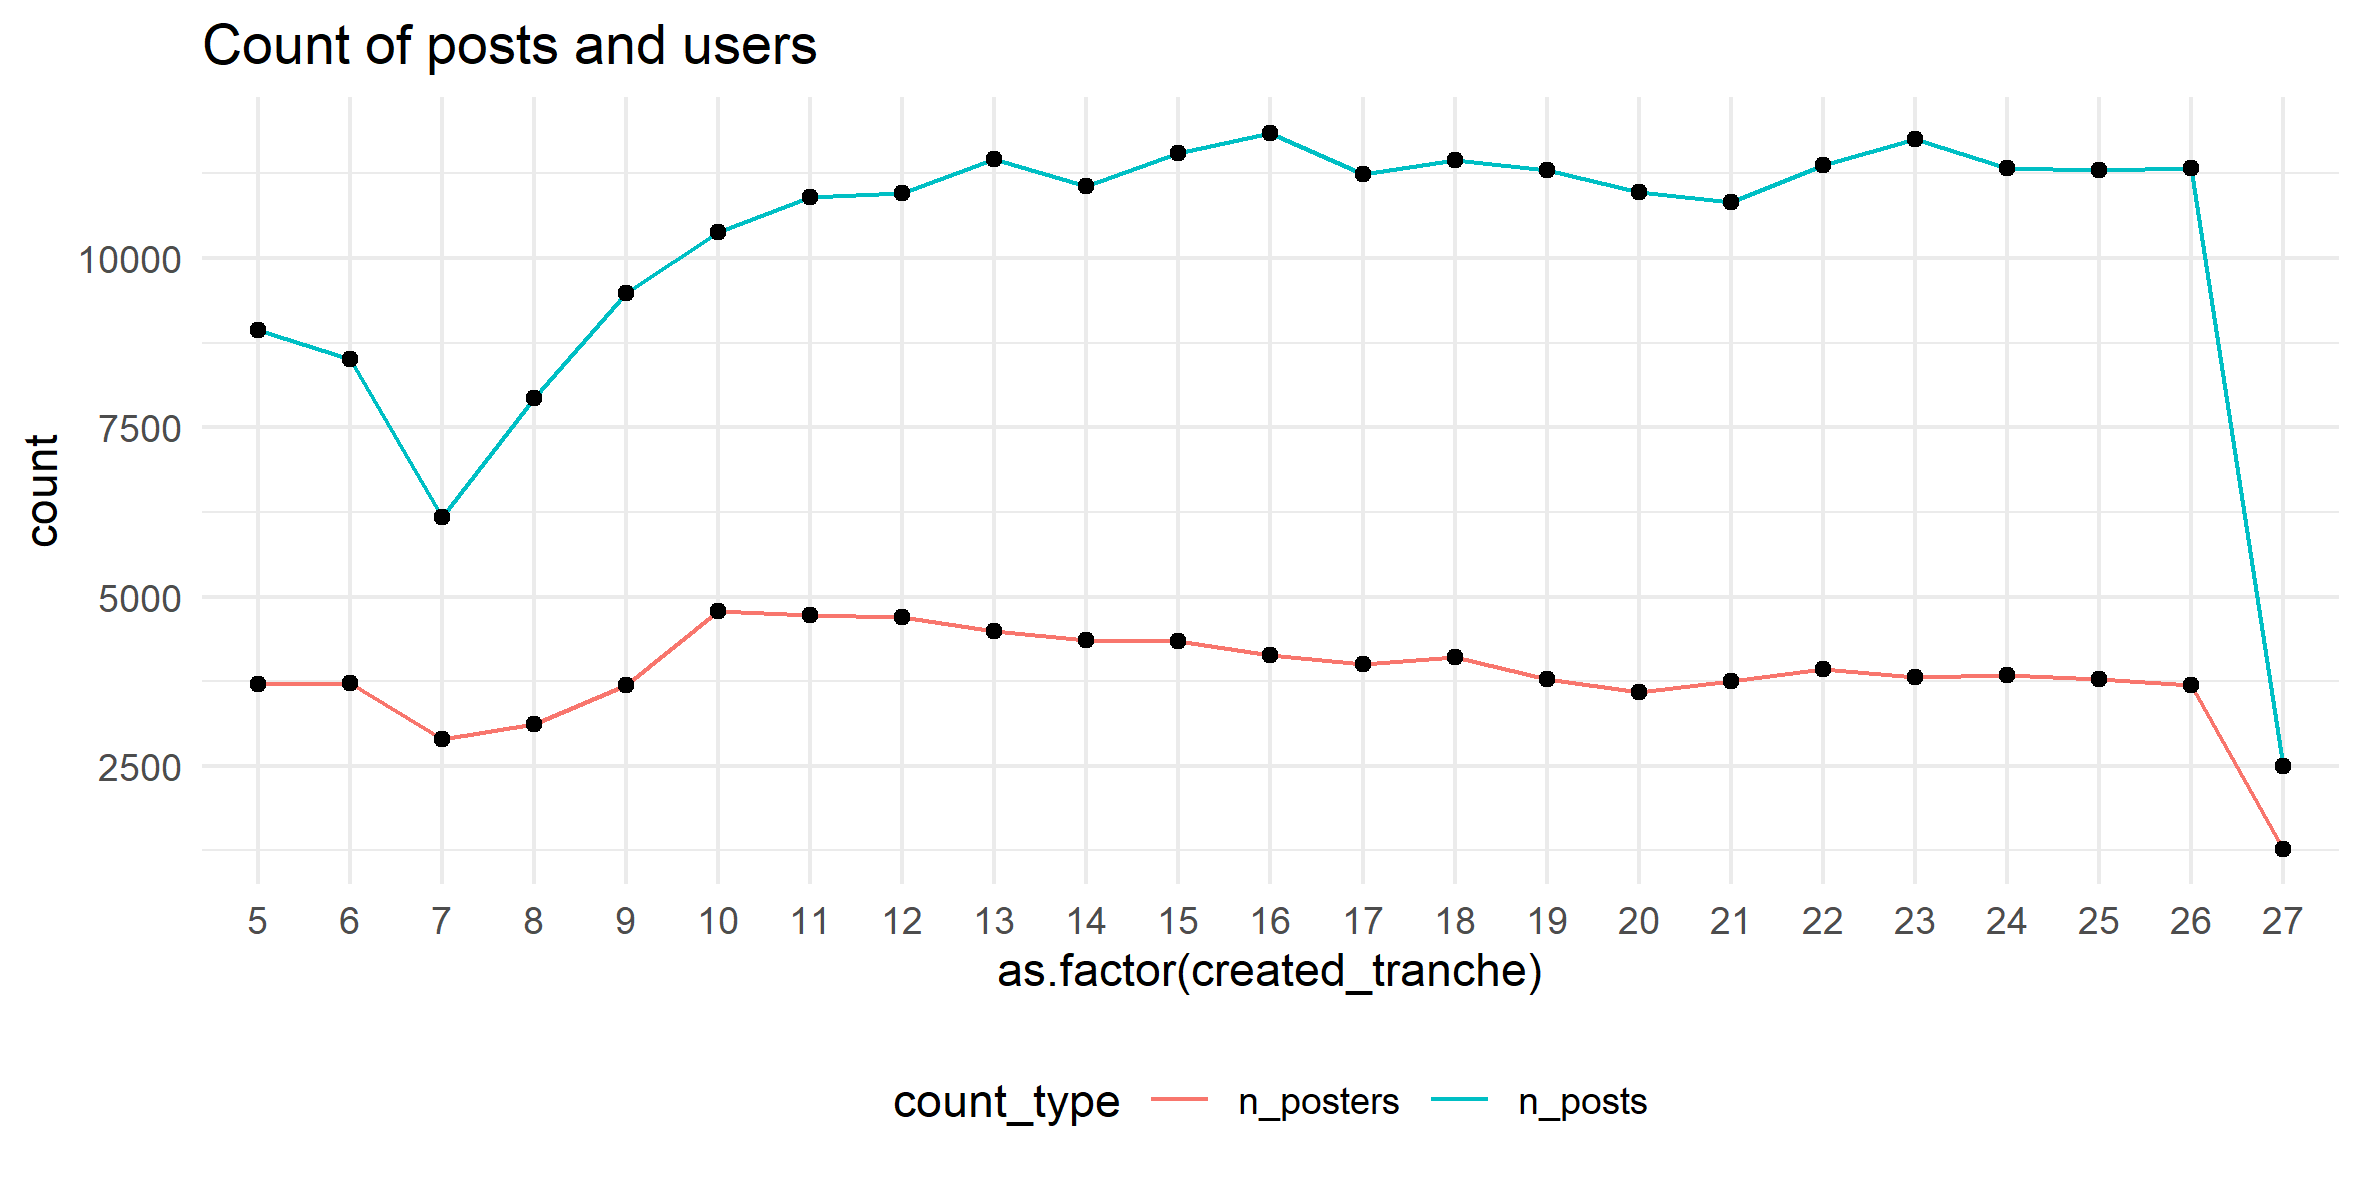
\includegraphics[width=\linewidth]{figures/sub_ts.png}
    \caption{Count of posts and posters for Snapshot Language Models.}%

    \label{fig:sub_stats}%

\end{figure}

% \subsection*{Identifying Elite-users}

% To identify elite users in each window of the subreddit, I construct an interaction network of users. This is the graph of users who have replied to each other, and is constructed from all posts and comments for a given window. It is important to note that only direct replies are considered as a form of interaction. That is, if user B replies to A, and C replies to B, the constructed graph would be:

% \begin{figure}[h]
% \centering
% 
\includegraphics[width=0.5\textwidth]{figures/int_graph.png}
% \caption{Sample Interaction Graph}
% \end{figure}

% The interaction graph is a directional network and weighted by the number of interactions between two users. Elite users for each window are identified using Bonacich centrality, which measures status within the network \citep{bonacich_power_1987}. I examine the top $0.1\%$ of users.

\subsection*{Word Embeddings to describe Context \& Change in Community Discussions}

To describe the context surrounding topics of interest in the community, I construct word embedding models for each period using skip-grams with negative sampling using Python's \texttt{gensim}\citep{rehurek_lrec} library. The high-dimensional corpus of text is reduced to lower dimension where each word $w_i$ is represented by a vector $\textbf{w}_i$ of size $k$ \citep{kozlowski_geometry_2019}. The skip-gram approach captures the nature of co-occurence between words and phrases. Semantic similarity -- and divergence, by extension -- between two words is measured using the cosine similarity between the two word vectors representing them \citep{hamilton_diachronic_2018}. I retain all posts and comments for this method.

To compare the divergence of words from different time-periods, we need to ensure that the word vectors are aligned to the same coordinate axes. I use the Procrustes alignment method developed by Hamilton et al.  \citep{hamilton_diachronic_2018}. For $p$ time-periods, we take the common vocabulary across these periods and obtain the optimal rotational alignment that preserves cosine similarities. After alignment, we can use the adjusted word vectors to compute semantic divergence, i.e. how the context of a word has shifted over time. This is measured using the cosine distance between the word vectors in time $t, t + \Delta$: $cosineDist(\textbf{w}_t, \textbf{w}_{t+\Delta})$. \citep{hamilton_diachronic_2018}

Additionally, I construct semantic dimensions for issues to track how certain the context surrounding specific issues shift over time. For each dimension, I take the normalized sum of antonym pairs to create a bi-directional vector to project word vectors onto. \citep{kozlowski_geometry_2019} The cosine-similarity of word vectors with these dimensions tells us where the word lies on the spectrum created by that dimension. 

I create six dimensions of interest, which are enumerated below. The complete list of antonym pairs used to construct them is provided in Table \ref{tab:dim-table}.

\begin{enumerate}
    \item Security: How closely do entities relate to issues of safety and security. Eg: Are candidates \textit{strong} or \textit{weak} on crime?
    \item Trade: To capture the context around trade issues -- \textit{local} protectionism vs. \textit{global} free trade.
    \item Ideology: Create a dimension to quantify the ideological spectrum between \textit{left} and \textit{right}, \textit{conservative} and \textit{liberal}.
    \item Region: Are the issues of the party focused on cities and the \textit{coast}, or are they referring to the \textit{heartland}?
    \item Economy: Is the party associated with the \textit{rich} and the elite, or do they speak to the \textit{poor} in America.
    \item Race: Where are candidates positioned on questions of race and immigration.
\end{enumerate}

Additionally, I restrict my analysis of these semantic dimensions to four distinct windows. This is to simplify the attempt to explain sifts within the same dimension driven by events. These windows are selected to indicate vital time periods in the Trump presidency. These periods include:  
\begin{enumerate}
	\item Super Tuesday, March 2016: A major victory for Donald Trump in the Republican Primary in key states on Super Tuesday, which made him the front-runner for the nomination. In the run-up to Super Tuesday, he moved from being an outside candidate to a viable candidate, fleshing out his policies and campaign rhetoric.

	\item General Elections, November 2016: Donald Trump beats Hillary Clinton in an upset victory by the slimmest of margins. Coverage in the final days was heavily influenced by investigations into Clinton's e-mail server, precipitated by a letter from FBI director James Comey to Congress about newly discovered material days before the election. 

	\item The first quarter of the presidency, February - March 2017.  

	\item `Unite the Right' rally in Charlottesville, Virginia, August 2017: This was a white-supremacist rally conducted in response to the removal of Confederate monuments by local governments. The rally served as a unifying event for the American white-nationalist movement, and attracted counter-protestors. It turned violent after clashes between the two groups, and on Day 2, a white supremacist deliberately drove his car into the counter-protestors, killing one of them. 
\end{enumerate}  

\begin{table}[t]
\caption{Antonym pairs used to construct Semantic Dimensions}
\label{tab:dim-table}
\resizebox{\textwidth}{!}{%
\begin{tabular}{@{}llrlll@{}}
\toprule
Security & Trade & Ideology & Region           & Economy       & Race         \\ \midrule
safe - vulnerable & local - global & right - left           & rural - urban & rich - poor      & white - black        \\
strong - weak     & tariff - free  & conservative - liberal & town - city   & advantage - need & american - immigrant \\
         &       &          & interior - coast & equity - loan & close - open \\ \bottomrule
\end{tabular}%
}
\end{table}